% ---
% Arquivo com a execução do Trabalho de Conclusão de Curso dos aluno
% Daniel Noriaki Kurosawa 
% da Escola Politécnica da Universidade de São Paulo
% ---
	\chapter{Execução e Resultados obtidos}\label{cap-execucao}
	Ete capítulo apresenta as atividades realizadas resultados atingidos, obtidos a partir da especificação do sistema e da metodologia de trabalho adotada.
	
	\subsection{Controle abre-fecha e rotação da garra}\label{subsec-garra}
	Primeiramente, foi feito o estudo de movimentação garra e de seu controle, uma vez que seu controle é totalmente independente da posição do braço. Para os testes, os comandos foram gerados à partir de uma placa Arduino Mega 2560(\autoref{fig_garra}).\par

	\begin{figure}[h]
	\caption{\label{fig_garra} Garra do braço robótico }
	\begin{center}
		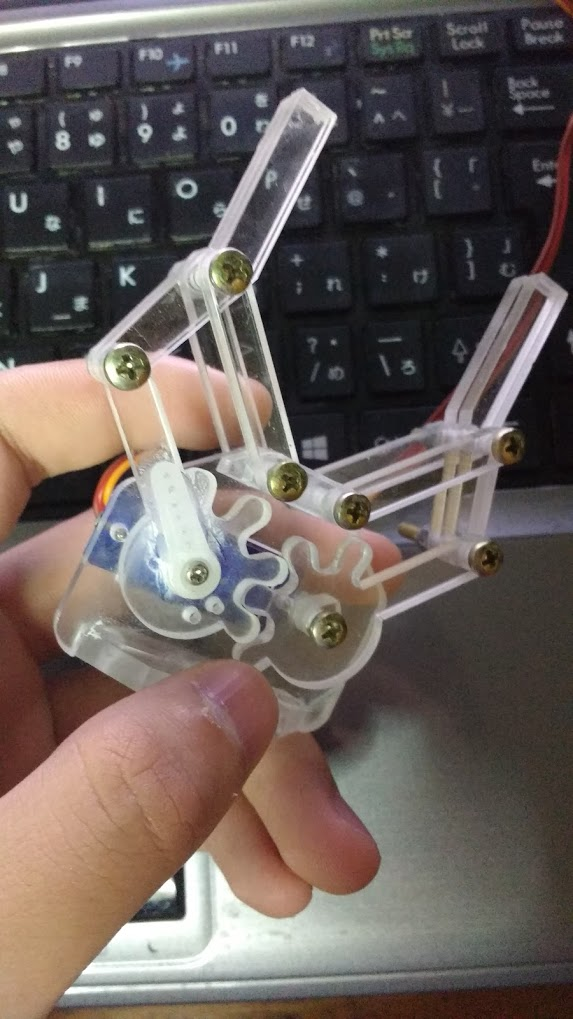
\includegraphics[width=50mm,scale=0.5]{IMG_20160523_203903430.jpg}	
	\end{center}
	\legend{Fonte: Autor}
\end{figure}

	\subsection{Modelagem de movimentação do braço}\label{subsec-modelagem}
	Foi feita a modelagem de todos os movimentos possíveis para o braço robótico para posterior uso como referência durante o projeto.\par
	\subsubsection{Modelagem inicial}\label{subsubsec-modelageminic}
	Inicialmente, foi feita a modelagem para dois motores (ombro e cotovelo), e gradualmente o modelo foi melhorado(\autoref{fig-mov2D}). \par
	\begin{figure}[!htb]
	\caption{\label{fig-mov2D} Coordenadas X-Y para todos os valores de theta1 e theta2 }
	\begin{center}
		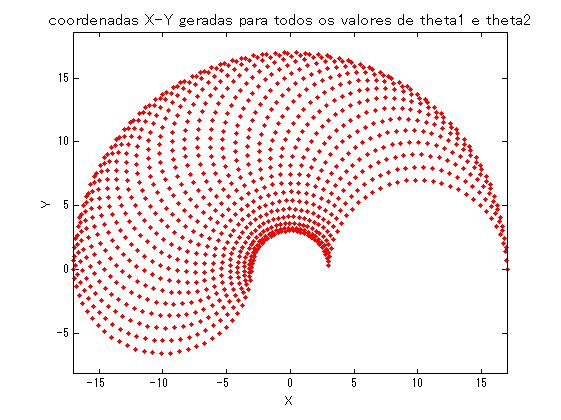
\includegraphics[width=100mm]{2dof.jpg}	
	\end{center}
	\legend{Fonte: Autor}
	\end{figure}

	\subsubsection{Modelagem da movimentação do braço para os motores correspondentes ao ombro, cotovelo e rotação do ombro do braço}\label{subsubsec-modelagem3m}

	O modelo foi ampliado para incluir o terceiro dos 4 motores de movimento do braço(\autoref{fig-mov3D}).\par
	\begin{figure} [!htb]
	\caption{\label{fig-mov3D}  Coordenadas X-Y-Z para todos os valores de theta1, theta2 e theta3 }
	\begin{center}
		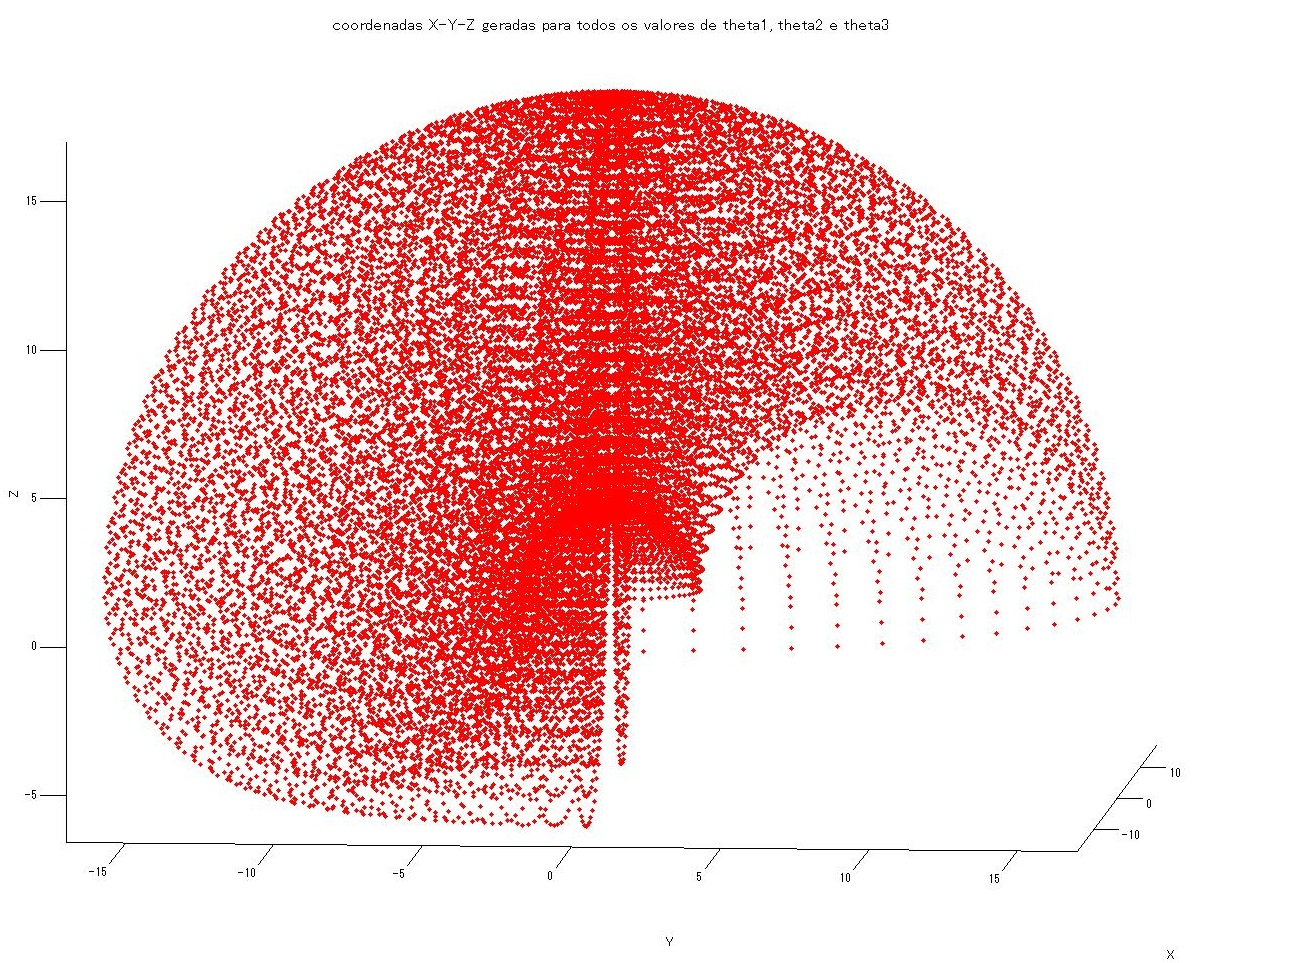
\includegraphics[width=100mm]{3dof.jpg}	
	\end{center}
	\legend{Fonte: Autor}
	\end{figure}

	\subsubsection{Modelagem da movimentação do braço para os motores correspondentes ao ombro, cotovelo, rotação do ombro e pulso do braço}\label{subsubsec-modelagem4m}

	Inclusão do quarto e último motor referente ao braço, completando o modelo a ser utilizado(\autoref{fig-mov4D}).\par

	\begin{figure}[htb!]
	\caption{\label{fig-mov4D}  Coordenadas X-Y-Z para todos os valores de theta1, theta2, theta3 e theta4 }
	\begin{center}
		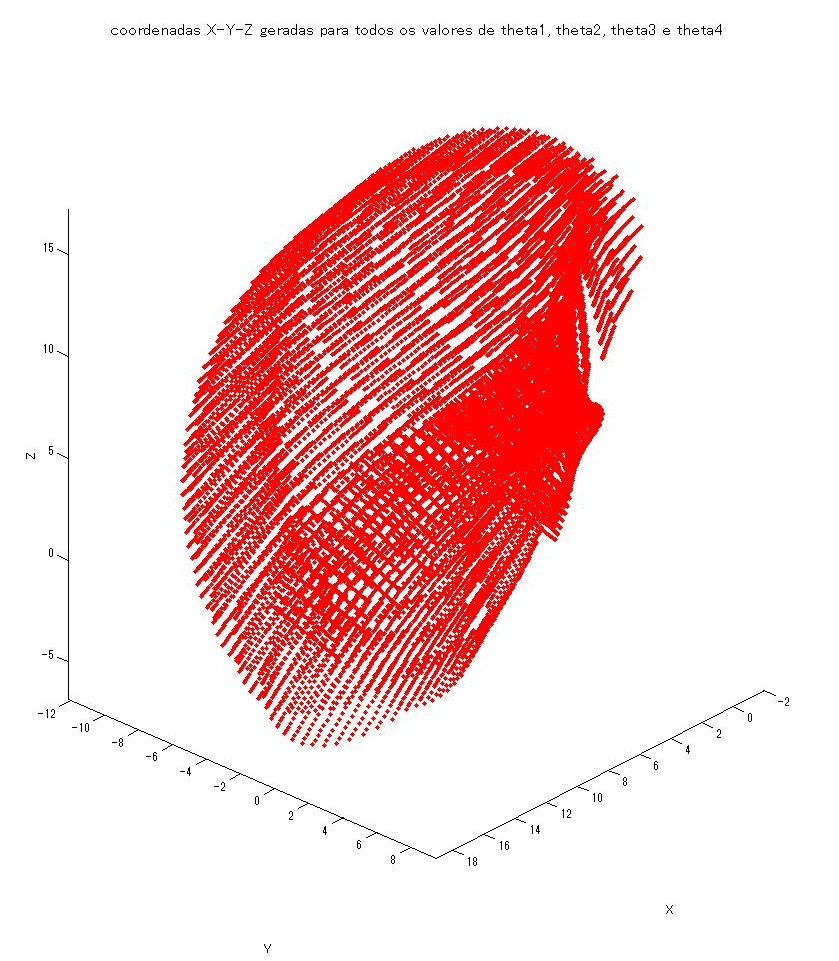
\includegraphics[width=100mm]{4dof.jpg}	
	\end{center}
	\legend{Fonte: Autor}
\end{figure}

\subsection{Aquisição de imagens pela camera}\label{subsec-cameras}

Figura 17: Imagem das cameras estereoscópicas
A aquisição das imagens foi feita usando um computador Raspberry Pi rodando o sistema operacional Raspbian Jessie.\par 

Para isso, foram testados os programas motion, gstreamer e Mjpg-Streamer. A seguir,  é feita uma comparação dos programas:
motion: baixa complexidade de configuração, taxa de captura baixa, alto consumo de capacidade de processamento. Foi logo descartado
Gstreamer: alta complexidade para configuração inicial, taxa de captura moderada, alto consumo de capacidade de processamento, não amigável ao uso de duas câmeras.\par
mjpg-Streamer: Configuração inicial de dificuldade moderada, taxa de captura adequada quando configurado para modo de baixa resolução.
Após a escolha do programa, foi feito o estudo para a captura em tempo real de duas câmeras ao mesmo tempo. Para isso, foi primeiro feito o teste para duas instâncias do programa rodando ao mesmo tempo, após ajuste de taxa de captura e resolução provou-se que o programa mantinha-se estável o suficiente para aplicação. (\autoref{fig_cameras}).\par

\begin{figure}[h!]
	\caption{\label{fig_cameras}  Imagem obtida pelas câmeras estereoscópicas usando mjpg-streamer}
	\begin{center}
		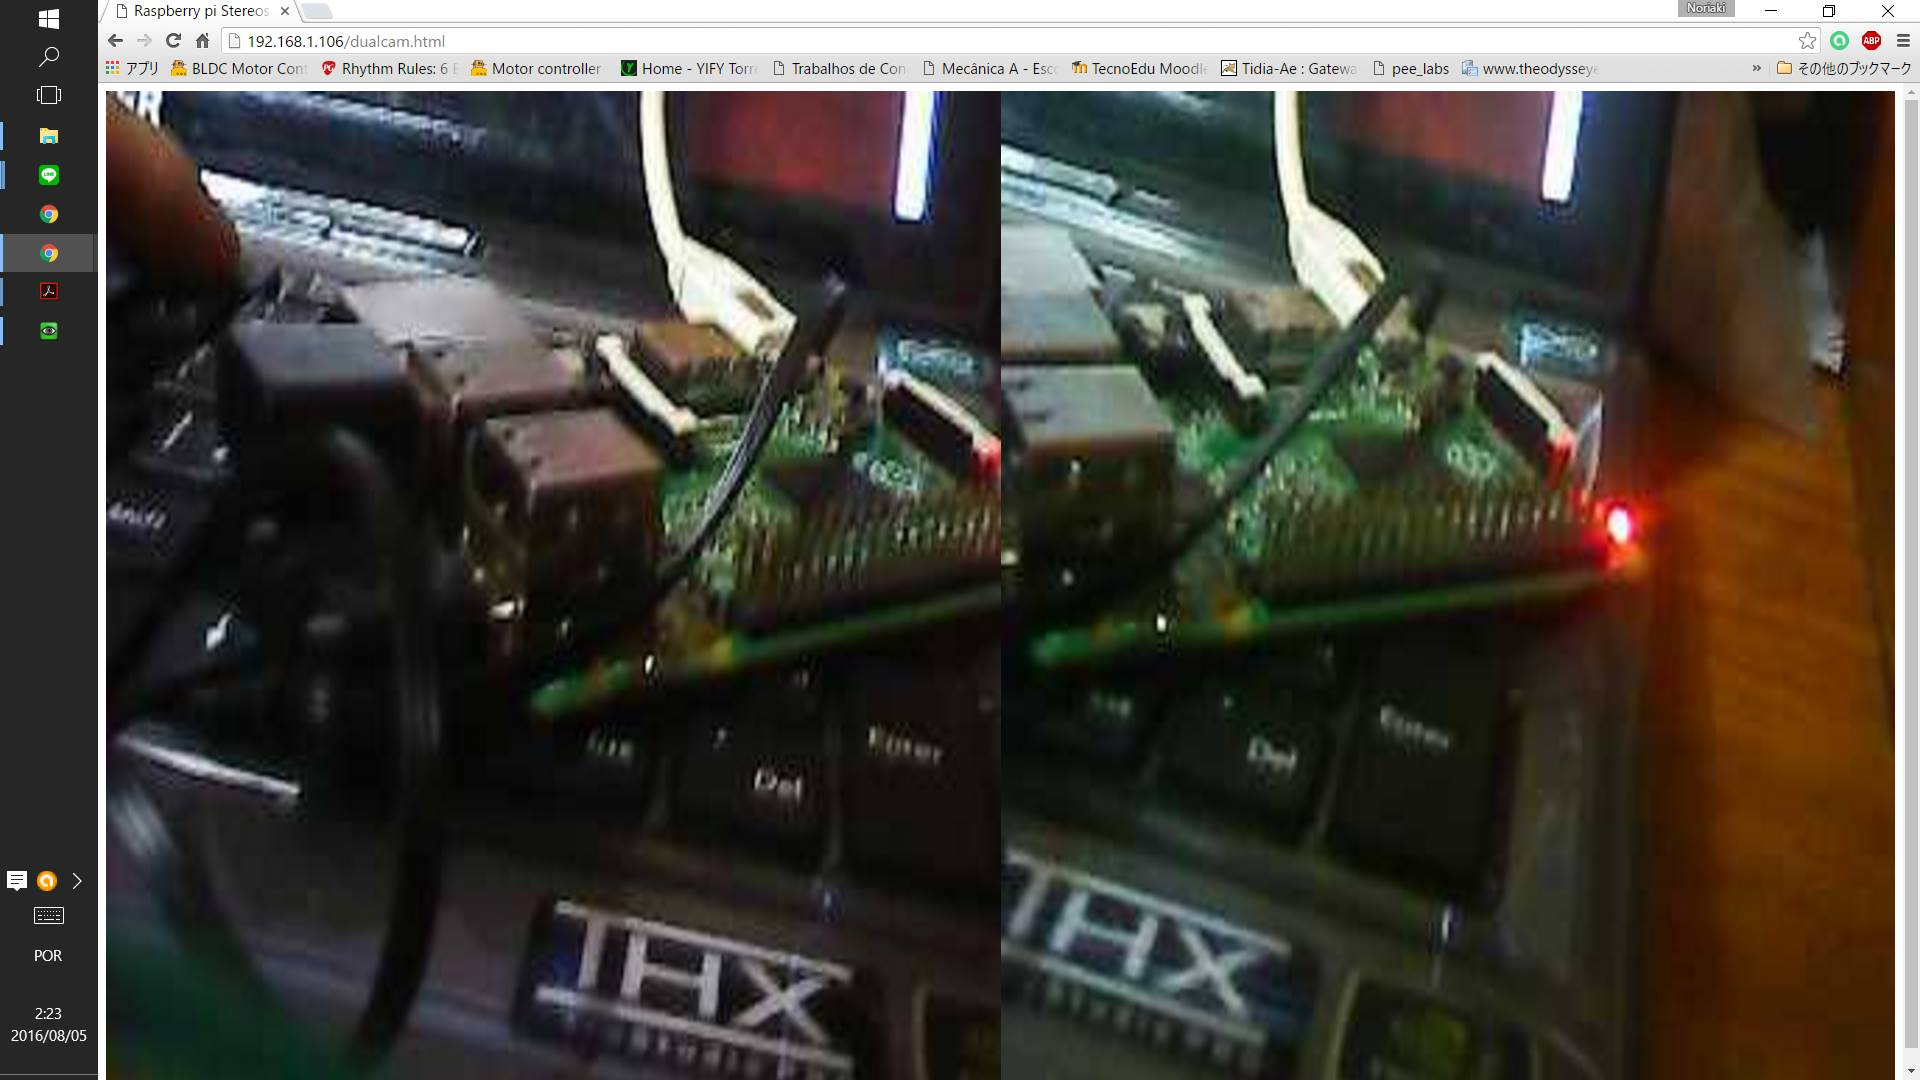
\includegraphics[width=100mm]{13898174_1266308583399952_1266040180_o.png}	
	\end{center}
	\legend{Fonte: Autor}
\end{figure}




\subsection{Montagem do sistema de motores e controle dos motores da câmera}\label{subsec-motores-camera}

Após a configuração das câmeras, foi feita a montagem de sua base com motores, que pode ser vista abaixo(\autoref{fig_camera_mount}): 

\begin{figure}[h!]
	\caption{\label{fig_camera_mount}  Montagem das câmeras estereoscópicas}
	\begin{center}
		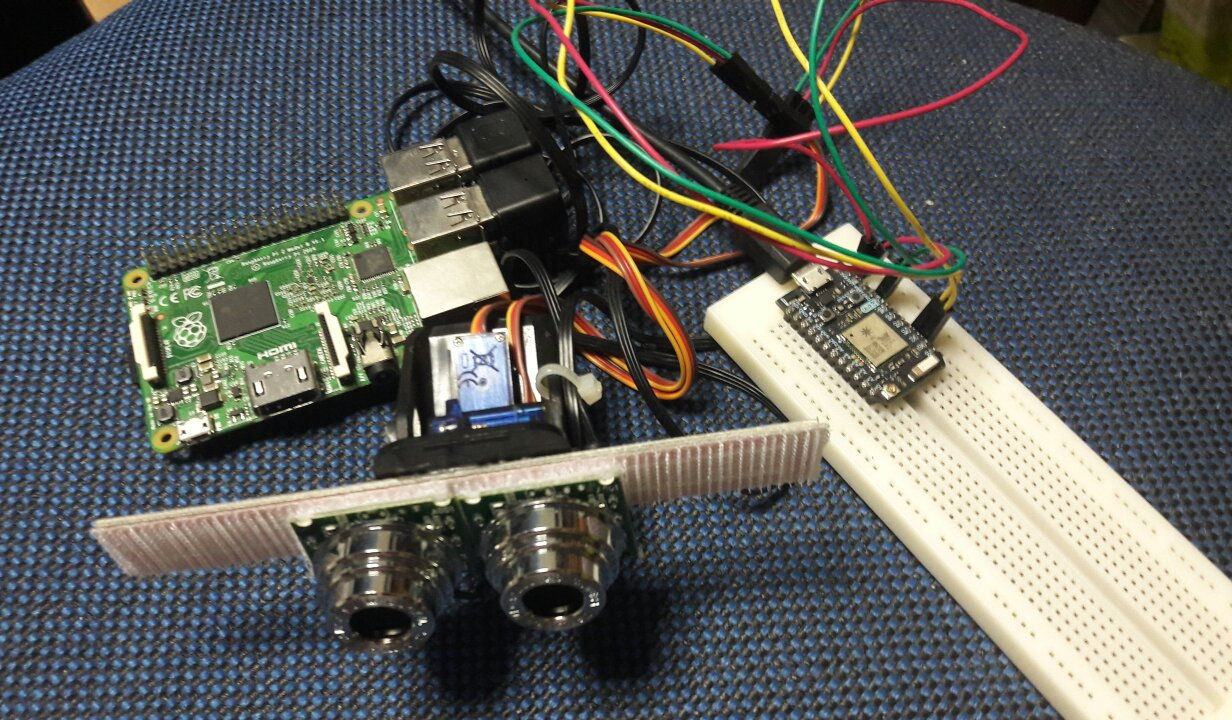
\includegraphics[width=100mm]{14407821_1315291101835033_240409903_o.jpg}	
	\end{center}
	\legend{Fonte: Autor}
\end{figure}

Após a montagem, foi feita a configuração de duas placas Particle Photon que foram utilizadas como transmissor e receptor, devido ao seu tamanho e peso reduzidos e ao fato de possuir uma antena WiFi já embutida.
Para a captura dos movimentos da cabeça do usuário, decidiu-se acoplar um giroscópio externo aos óculos de realidade virtual, de modo que o projeto não dependesse de formas de captura de movimentos específicas para cada modelo de óculos.\par
\begin{figure}[h!]
	\caption{\label{fig_vrglasses}  Óculos de realidade virtual com destaque para o giroscópio externo}
	\begin{center}
		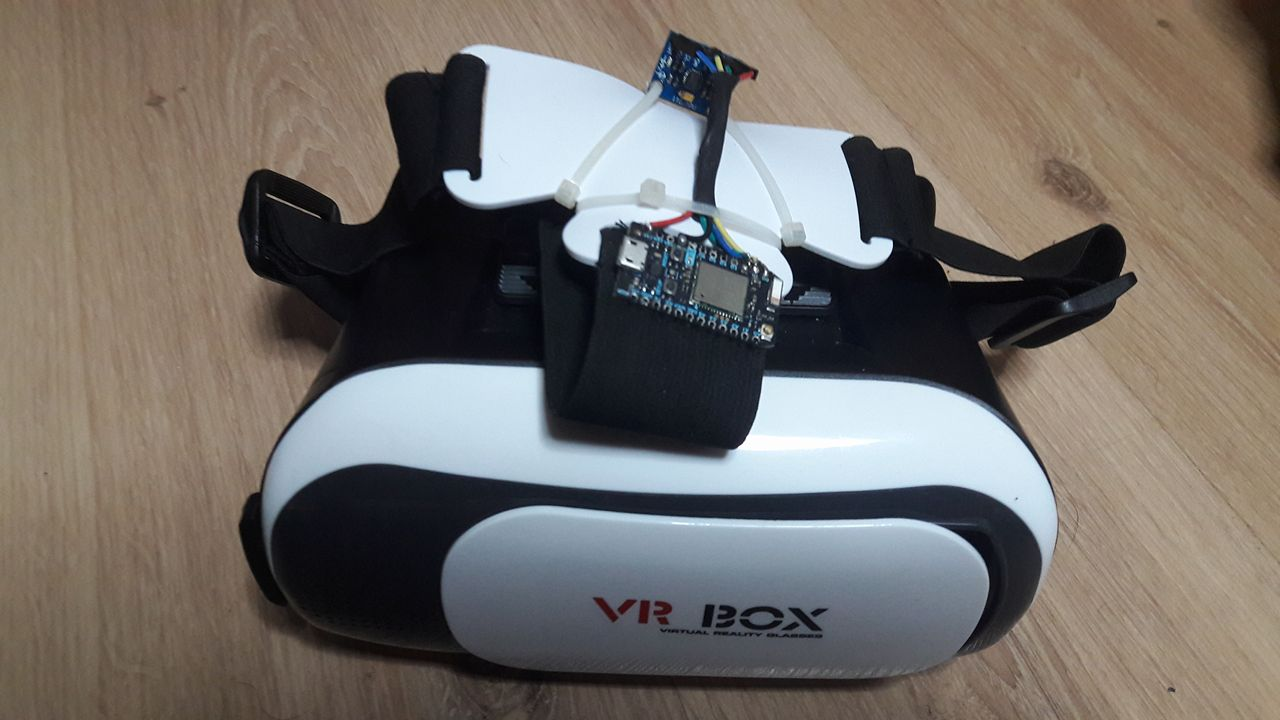
\includegraphics[width=100mm]{14424070_1315290465168430_612088294_o.jpg}	
	\end{center}
	\legend{Fonte: Autor}
\end{figure}
Para o transmissor, foram realizadas duas versões de código.
Inicialmente, foi  escrito um código usando-se a saída do giroscópio e realizando as conversão usando-se como base o algoritmo descrito em \cite{debra}. Este código era altamente dependente da posição inicial do giroscópio, que era usada para uma rotina de calibragem inicial.\par

A segunda versão do código foi realizada usando-se bibliotecas específicas ("MPU6050/I2Cdev.h" e "MPU6050/MPU6050\_6Axis\_MotionApps20.h") traduzidas de arduino, que fazem uso de algoritmos internos ao giroscópio para a calibragem , tornando-a mais rápida e precisa \par

Para o receptor, foi feita uma única versão, responsável por receber os ângulos de rotação e transmiti-los aos dois motores na base da câmera 
A transmissão dos dados atualmente se dá via protocolo UDP em uma rede local.\par

\subsection{ Captura de ângulos usando Processing}\label{subsec-Processing}
\begin{figure}[h!]
	\caption{\label{fig_processing}  Imagem obtida pelas câmeras estereoscópicas}
	\begin{center}
		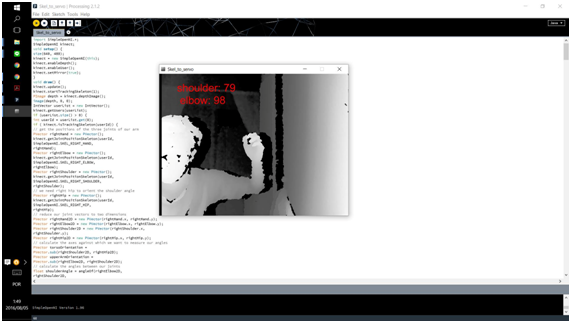
\includegraphics[width=100mm]{processing.png}	
	\end{center}
	\legend{Fonte: Autor}
\end{figure}
Foi utilizado inicialmente a linguagem Processing (baseada em Java), usando-se da bibliotenca OpenNI para a captura dos movimentos. No entanto, devido a baixa precisão da captura usando a biblioteca, essa abordagem foi abortada.\par


\subsection{ Captura de ângulos usando Visual C\#}\label{subsec-visualCsharp}
A programação foi realizada em Visual C\# usando-se como base o exemplo de captura e visualização de esqueleto do Microsoft Kinect 1.8 fornecido pela Microsoft, ao qual foram adicionadas funcionalidades necessárias ao projeto. No estado atual, o programa pode além de exibir o esqueleto com as juntas do usuário, capturar os ângulos do braço do usuário e exibi-los como números, para que seja feito o teste de coerência dos dados a serem enviados(\autoref{fig_visualcsharp}).\par
\begin{figure}[h!]
	\caption{\label{fig_visualcsharp}  Captura de ângulos do braço humano usando Visual C\# e Kinect}
	\begin{center}
		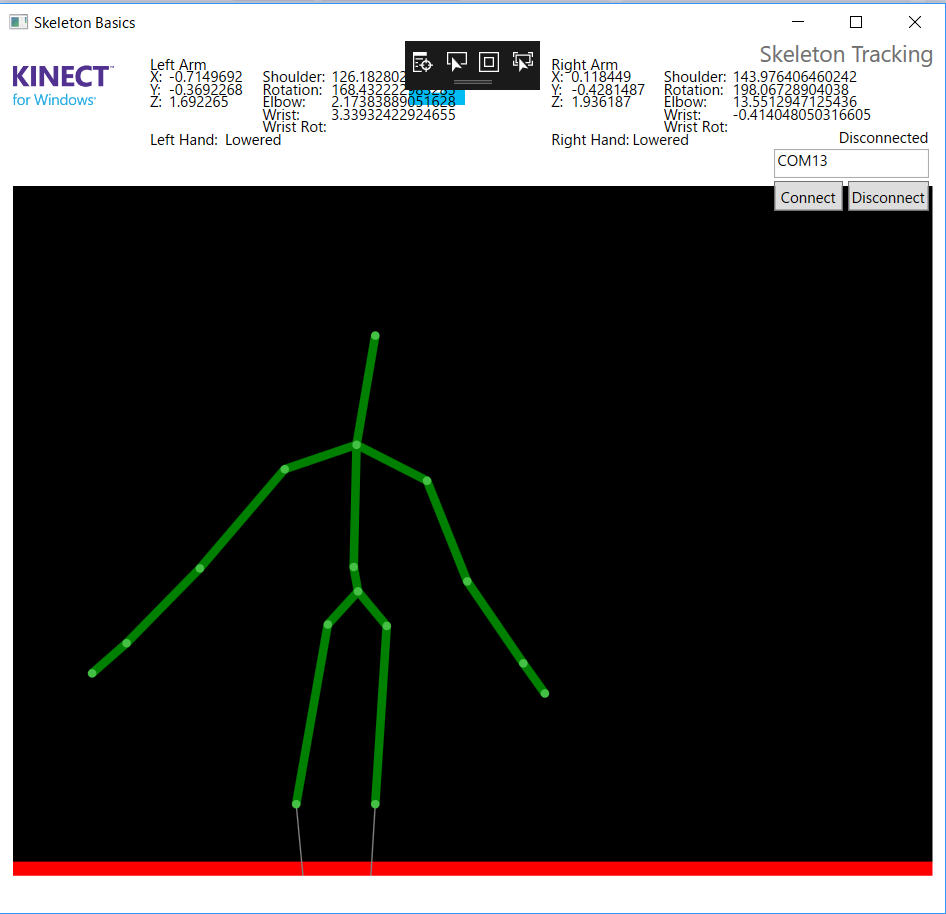
\includegraphics[width=100mm]{vbscreen.png}	
	\end{center}
	\legend{Fonte: Autor}
\end{figure}


\subsection{Controle dos servomotores via conexão serial usando Visual C\#}\label{subsec-VisualCsharpcontrol}
Foi feita a integração do controle dos servomotores com o programa responsável pela captura dos movimentos do usuário via conexão serial USB(\autoref{fig_base}). \par
\begin{figure}[h!]
	\caption{\label{fig_base}  Teste do motor da base do braço}
	\begin{center}
		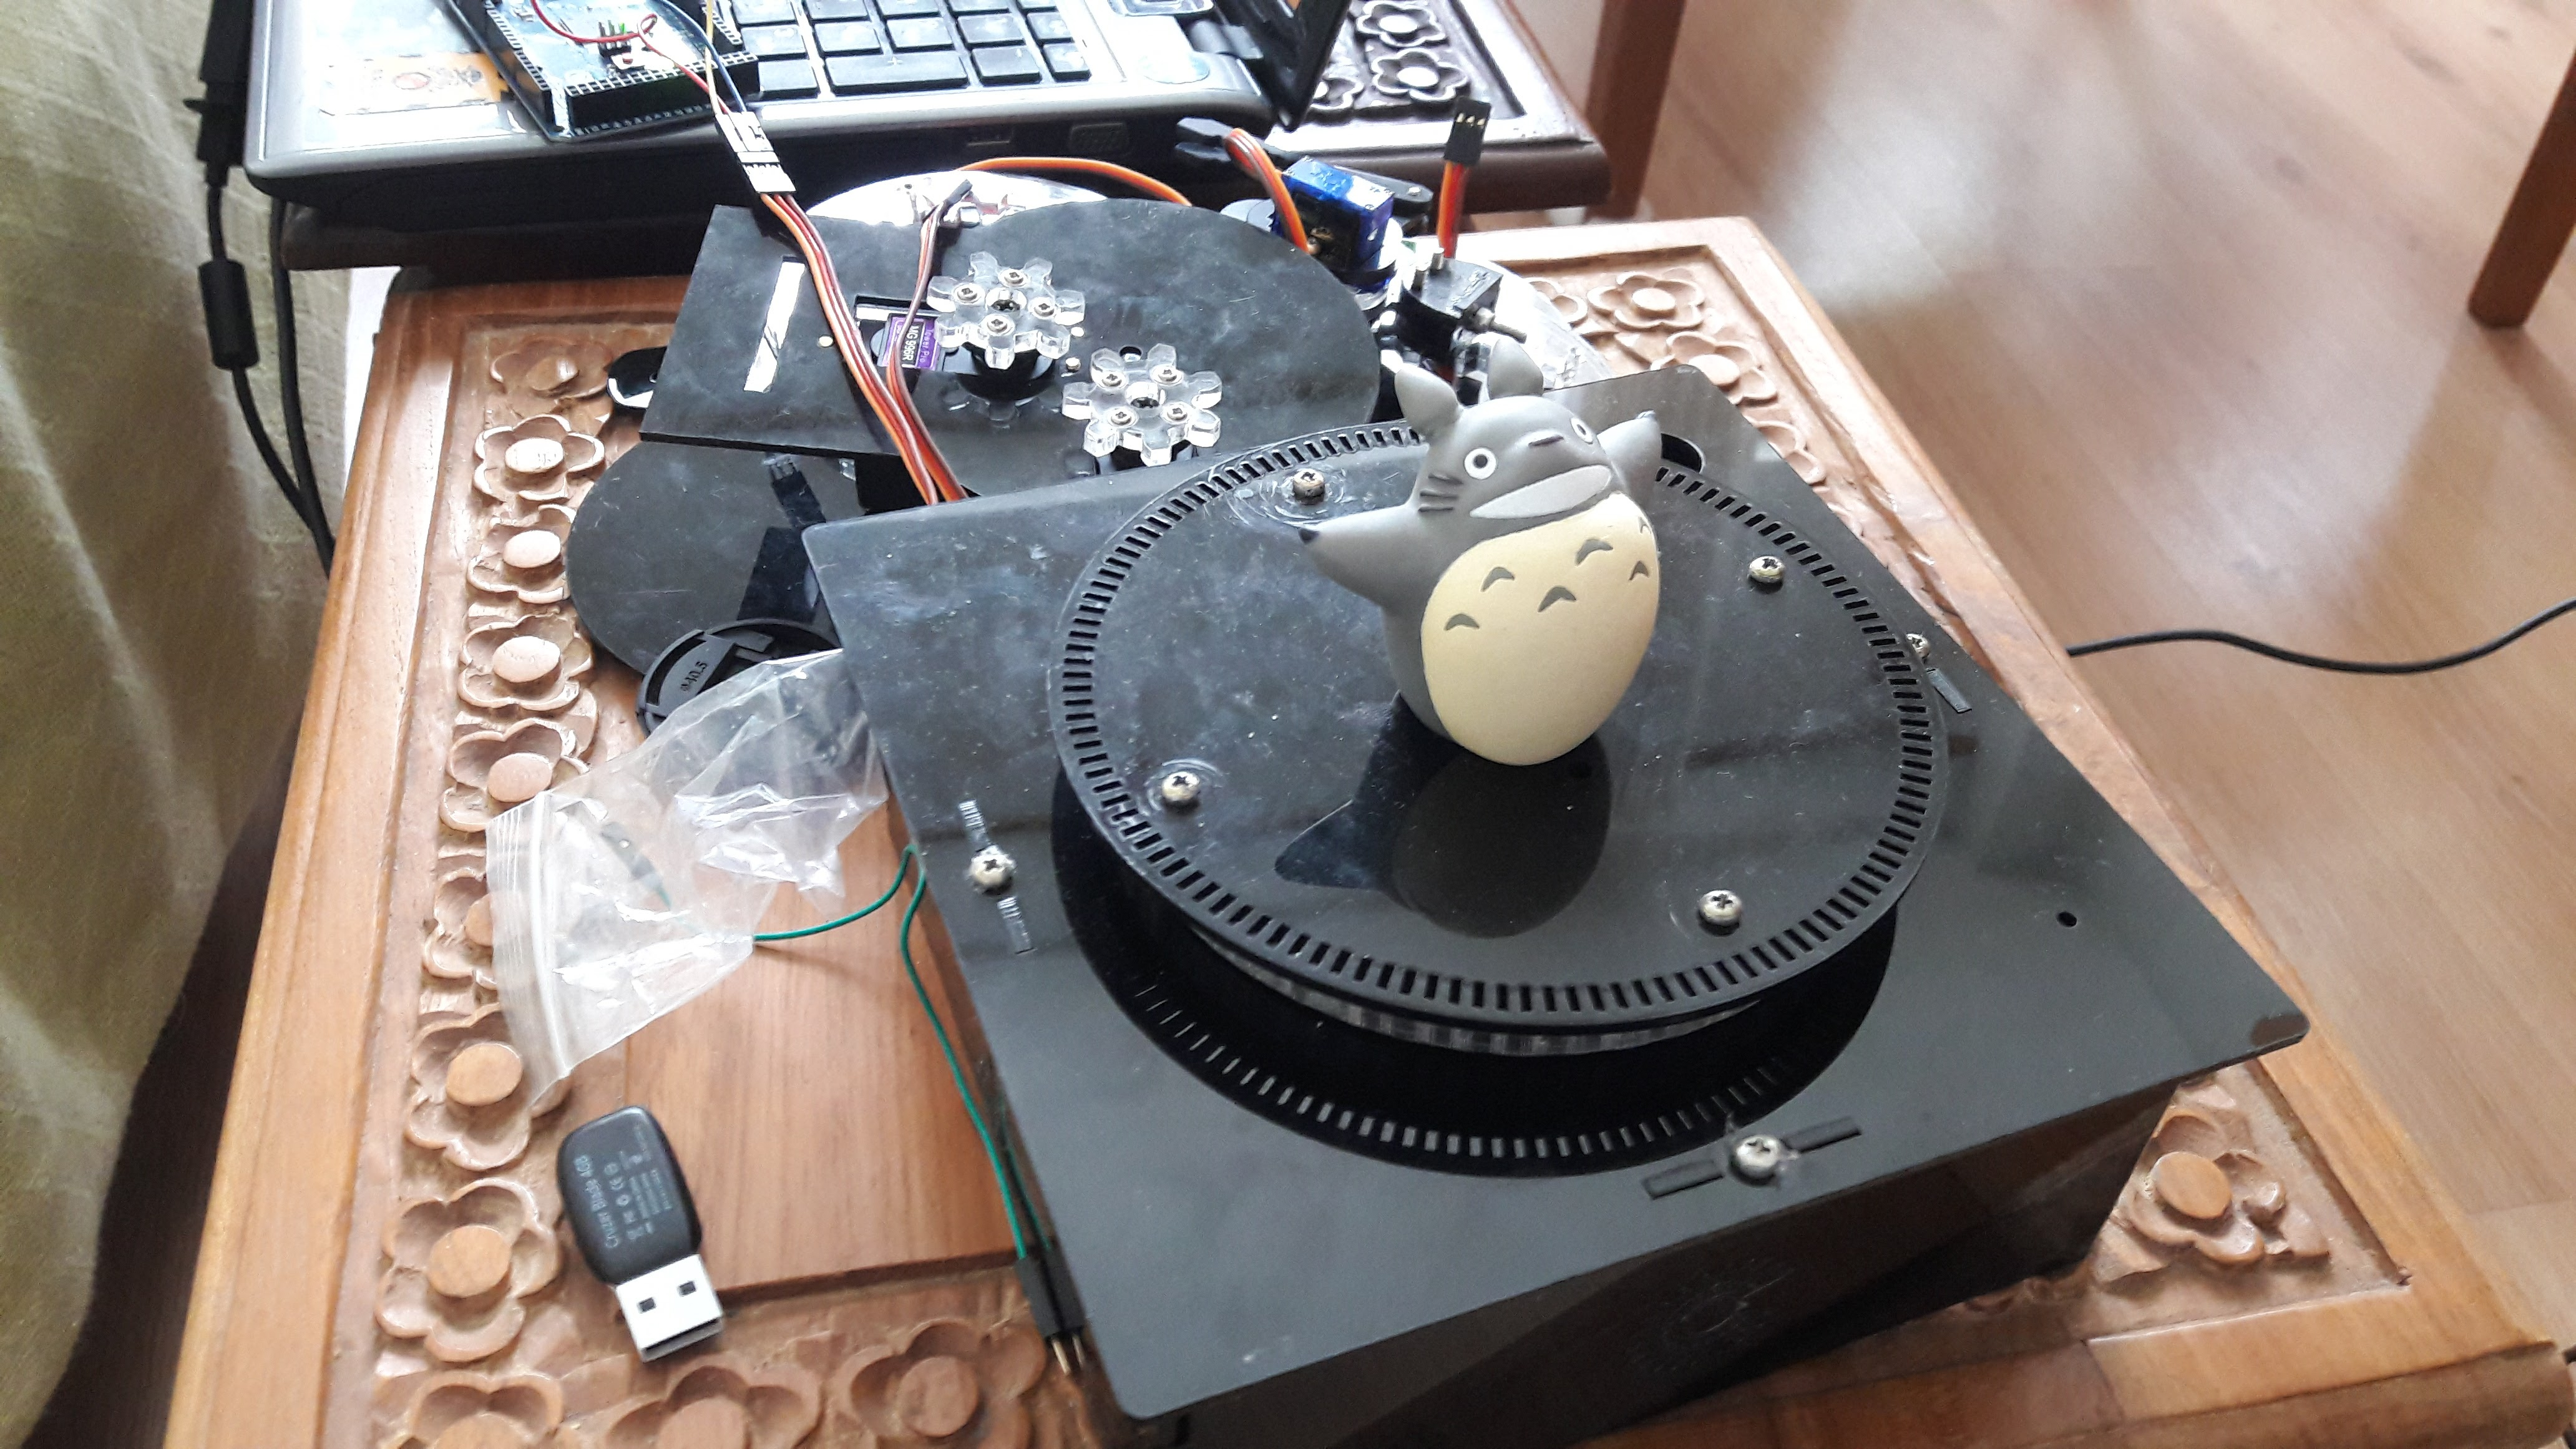
\includegraphics[width=100mm]{20161101_110237.jpg}	
	\end{center}
	\legend{Fonte: Autor}
\end{figure}
\subsection{Controle dos servomotores via conexão UDP usando Visual C\# e testes de integração}\label{subsec-all}
Nesta última etapa, foi feita a tradução do código para a SDK 2.0 do Kinect e a inclusão da funcionalidade WiFi ao programa. Com isso, foi feito de todo o sistema o teste em rede local, em que os atrasos de transmissão foram considerados irrelevantes (<0.1s)(\autoref{fig_integra;:ao}).\par
		\begin{figure}[h!]
			\caption{\label{fig_integrated}  Teste de integração}
			\begin{center}
				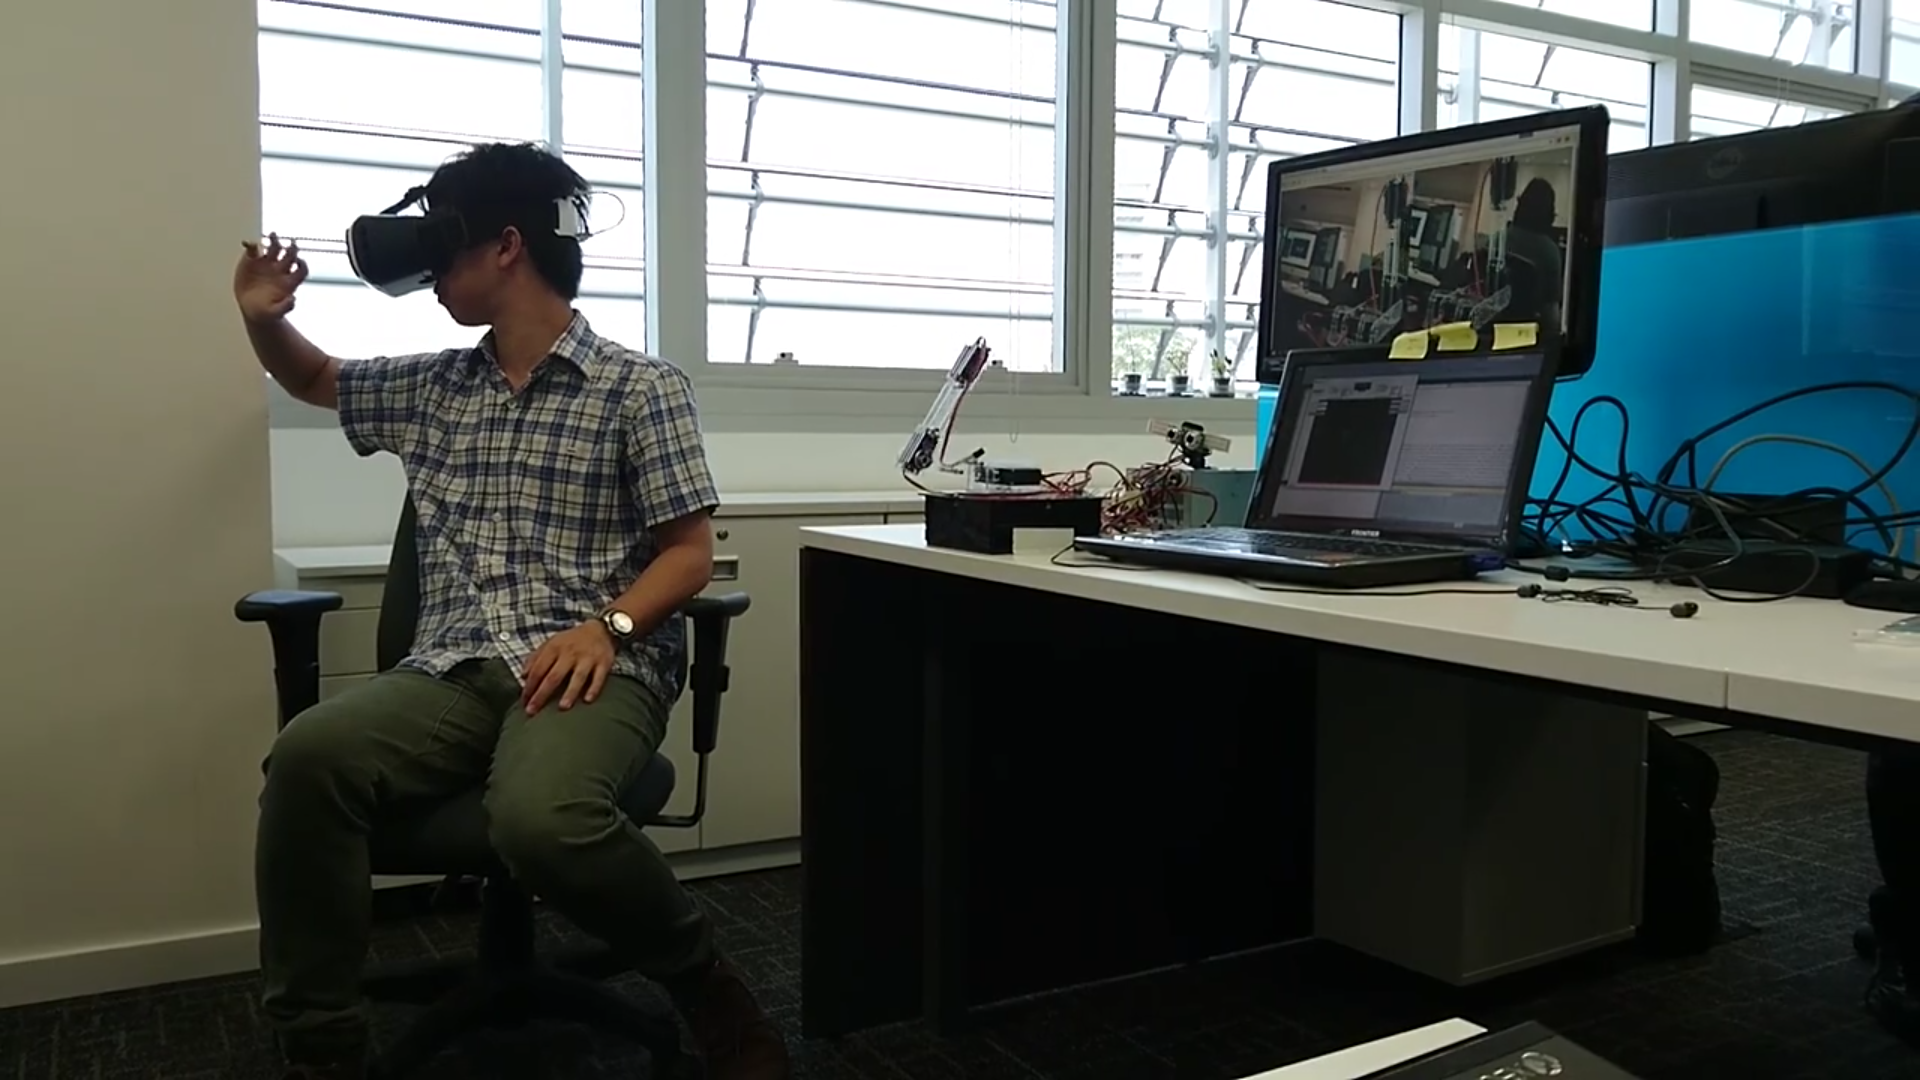
\includegraphics[width=100mm]{integrated.png}	
			\end{center}
			\legend{Fonte: Autor}
		\end{figure}

\section{Resultados}\label{sec-resultados}	
À partir da execução do projeto, foi possivel concluir que existe um grande espaço para o desenvolvimento deste tipo de projeto em aplicações futuras.\par
Foi constatado que o sistema de câmeras, apesar da baixa resolução do hardware utilizado, é capaz de fornecer uma razoável noção de profundidade, e aliado com a sua capacidade de seguir a movimentação do usuário, tem aplicações comerciais imediatas.\par
Percebeu-se no entanto, que existe uma baixa resistência a ruídos por parte do sensor óptico Microsoft Kinect que apresentava altas taxas de erro de leitura em testes com mais de um ser humano em tela. \par
 É relevante notar também que o mesmo apresentou dificuldade na leitura do usúario quando este se encontrava de perfil em relação ao sensor, o que, aliado a falta de noção espacial do usuário em relação ao próprio corpo quando no modo de imersão, pode causar dificuldades na interação com o ambiente remoto, com o possível descontrole do braço.\par
 É possível assim, concluir que ainda são necessárias melhorias antes de tal abordagem ser aplicável a usos comerciais.